\documentclass[pra,
aps,
twocolumn,
superscriptaddress,
groupedaddress,
nofootinbib,
reprint
]{revtex4-1}

% PACKAGES
\usepackage{amsmath,amsfonts, amssymb, amsthm}
\usepackage{bm, bbm, physics, mathtools}
\usepackage{graphicx, subfigure}
\usepackage{xcolor, enumerate}
\usepackage{xifthen, hyperref}
\usepackage[capitalise]{cleveref}

\hypersetup{
	colorlinks=true,  
	linkcolor=blue,   
	citecolor=blue,   
	urlcolor=blue     
}

\newcommand{\crefrangeconjunction}{--}
\creflabelformat{figure}{(#2#1#3)}

% COMMENT NOTATION
\newcommand{\nick}[1]{{\color{red}#1}}
\newcommand{\ddd}[1]{\textcolor{blue}{#1}}

% ENVIRONMENTS
\newtheorem{theorem}{Theorem}
\newtheorem{proposition}[theorem]{Proposition}
\newtheorem{lemma}[theorem]{Lemma}
\newtheorem{definition}[theorem]{Definition}

% REFERENCES
\iffalse
\renewcommand{\eqref}[1]{Eq.~(\ref{#1})}
\newcommand{\figref}[1]{Fig.~(\ref{#1})}
\newcommand{\tabref}[1]{Tab.~(\ref{#1})}
\newcommand{\secref}[1]{Section~(\ref{#1})}
\newcommand{\appref}[1]{Appendix~(\ref{#1})}
\newcommand{\defref}[1]{Definition~\ref{#1}}
\newcommand{\lemref}[1]{Lemma~\ref{#1}}
\newcommand{\thmref}[1]{Theorem~\ref{#1}}
\fi

% SYMBOL DEFINITIONS
\renewcommand{\cal}[1]{\mathcal{#1}}

\newcommand{\reals}{\mathbb{R}}
\newcommand{\id}{\mathbbm{1}}
\newcommand{\idc}{1_{\rm{C}}}
\newcommand{\supf}{\mathfrak{c}}
\renewcommand{\tr}{{\rm{tr}}}
\renewcommand{\det}{{\rm{det}}}
\newcommand{\floor}[1]{\left\lfloor #1 \right\rfloor}
\newcommand{\ent}[2]{S\left( #1 \middle\vert\middle\vert #2 \right)}
\newcommand{\ents}{{\ent{\frac{m}{n}}{p}}}

\def\dummy{\ell}
\def\NN{n}
\def\mmf{i}
\def\nnf{n}
\def\mlt{m}
\def\ii{i}
\def\jj{j}
\def\kk{k}
\def\II{I}
\def\nn{n}
\def\tt{n'}
\def\mm{a}
\def\wp{u}
\def\wn{v}

\newcommand{\too}[1]{^{\otimes #1}}
\newcommand{\noisys}{\rho_{\rm{S}}}
\newcommand{\noisysn}{\rho_{\rm{S}}(\epsilon)^{\otimes \nn}}
\newcommand{\noisysN}{\rho_{\rm{S}}(\epsilon)^{\otimes \NN}}

\newcommand{\spanv}[1]{
    {{\rm{span}}\left\{#1\right\}}
}
\newcommand{\conv}[1]{
    {{\rm{conv}}#1}
}
\newcommand{\orb}[1]{
    {{\rm{orb}}(#1)}
}
\newcommand{\sn}[1]{
    {{\rm{sn}}\left(#1\right)}
}
\newcommand{\mana}[1]{
    {{\rm{mana}}\left(#1\right)}
}
\newcommand{\lc}[2]{
	{{\rm{L}}_{#1|#2}}
}

\newcommand{\bmx}{\bm{x}}
\newcommand{\bmy}{\bm{y}}
\newcommand{\bmz}{\bm{z}}
\newcommand{\bmu}{\bm{u}}
\newcommand{\bmw}{\bm{w}}
\newcommand{\bmo}{\bm{0}}
\newcommand{\bmd}{\bm{d}}
\newcommand{\bma}{\bm{a}}
\newcommand{\bmxi}{\bm{\xi}}
\newcommand{\bmg}{\bm{g}}

\newcommand{\zd}[1][]{
    \ifthenelse{\isempty{#1}}{
    {\mathbb{Z}_d} }{
    {\mathbb{Z}_{#1}}}
}
\newcommand{\hd}[1][]{
    \ifthenelse{\isempty{#1}}{
    {\cal{H}_d} }{
    {\cal{H}_{#1}}}
}
\newcommand{\pd}[1][]{
    \ifthenelse{\isempty{#1}}{
    {\cal{P}_d} }{
    {\cal{P}_{#1}}}
}
\newcommand{\cd}[1][]{
    \ifthenelse{\isempty{#1}}{
    {\cal{C}_d} }{
    {\cal{C}_{#1}}}
}
\newcommand{\spd}[1][]{
    \ifthenelse{\isempty{#1}}{
    {{\rm{Sp}}(2, \zd)} }{
    {{\rm{Sp}}(2, \zd[#1])}}
}
\newcommand{\gp}[1][]{
    \ifthenelse{\isempty{#1}}{
    {\rm{GP}_d} }{
    {\rm{GP}_{#1}}}
}
\newcommand{\stoch}[1][]{
    \ifthenelse{\isempty{#1}}{
    {{\rm{S}}_d(\bmd)} }{
    {{\rm{S}}_d(#1)}}
}
\newcommand{\stochw}[1][]{
    \ifthenelse{\isempty{#1}}{
    {{\rm{S}}_{d^2}(\W{\sigma})} }{
    {{\rm{S}}_{d^2}(#1)}}
}
\makeatletter
\def\W{\@ifnextchar[{\@with}{\@without}}
\def\@with[#1]#2{ 
    {{\rm{W}}_{#2}\left(#1\right)} }
\def\@without#1{ 
    {{\rm{W}}_{#1}} }
\makeatother

\newcommand{\T}{\cal{T}}
\newcommand{\Z}{\cal{Z}}

\newcommand{\C}{\cal{C}}
\newcommand{\E}{\cal{E}}
\newcommand{\J}{\cal{J}}
\newcommand{\R}{\cal{R}}
\newcommand{\D}{\cal{D}}
\newcommand{\F}{\cal{F}}
\renewcommand{\O}{\cal{O}}
\newcommand{\M}{\cal{M}}

\newcommand{\Fmax}{\F_{\rm{max}}}
\newcommand{\Omax}{\O_{\rm{}max}}
\newcommand{\Rmax}{\R_{\rm{}max}}
\newcommand{\Pis}{\Pi_{\rm{s}}}
\newcommand{\Pio}{\Pi_{\rm{o}}}

\newcommand{\cptp}{{\rm{CPTP}}}
\newcommand{\cpos}{{\rm{CP}}}
\newcommand{\so}{{\rm{SO}}}
\newcommand{\stab}{{\rm{STAB}}}
\newcommand{\spo}{{\rm{SPO}}}
\newcommand{\cspo}{{\rm{CSPO}}}
\newcommand{\rcu}{{\rm{RCU}}}
\newcommand{\tho}{{\rm{TO}}}
\newcommand{\cpwp}{{\rm{CPWPO}}}
\newcommand{\ru}{{\rm{RU}}}


\begin{document}



%%%%%%%%%%%%%%%%%%%%%%%%%%%%%%%%%%%%%%%%
\ddd{\subsection{Improving our abilities to include arbitrary output stabilizer states.}
The existing analysis works fine when the state $\tau'$ has stabilizer eigendecomposition (i.e. it's orthonormal basis is along the stabilizer directions...e.g. along $|0\>\<0|, |1\>\<1|$ in the Bloch sphere for a qubit). However it can lie inside the stabilizer polytope but not have such an eigenbasis. Therefore we'd like to include this fully general possibility.}

To do this we just need to analyse how the properties of the output state relate to the magnitudes of its Wigner components. Here let $\tau$ be a single full-rank stabilizer qutrit state -- we are really interested in the output state $\tau'$ but let's ignore primes for now....they just clutter expressions unnecessarily. For simplicity denote the Wigner components of the magic state as
\begin{equation}
	\w = (-v, u,u,u,u,u,u,u,u),
\end{equation}
and we index from $i=0$ to $i=7$, so that e.g. $w_0 = -v$ and $w_i = u$ for $i \ne 0$. Let $\t$ denote the Wigner distribution for $\tau$, so that
\begin{equation}
\t = (t_0, t_1,t_2, t_3, t_4,t_5,t_6,t_7),
\end{equation}
and we assume that $t_i >0$ for all $i$. We also note that using Clifford unitaries we can always choose to shift either the smallest entry of $\t$ or the largest entry of $\t$ to the $i=0$ slot. We might need to exploit this in a moment.

The rescaled distribution is then $\tilde{\w}\coloneqq (w_i/t_i)$, and we define $v_0 \coloneqq v/t_0$ and $u_i \coloneqq u/t_i$ for $i\ne 0$. We now need to consider the $n$--copy version of this, denoted $\tilde{\w}^{\otimes n}$, and determine how the largest component arises. A general component of $\tilde{\w}^{\otimes n}$ is given by,
\begin{equation}
\tilde{w}_{n,\alpha, i_1, \dots, i_8} = (-v_0)^{i_0} u_1^{i_1} u_2^{i_2} \cdots u_8^{i_8},
\end{equation}
with the assumption that firstly $n$ is always even, and the indices obeying the following conditions:
\begin{align}
0 &\le i_j \le n \mbox{ for each }j=0,1,\dots ,8 \nonumber \\
i_0+ i_1 &+ i_2 + \dots i_8 =n.
\end{align}
Now the largest entry must be positive, and so we require that $\alpha$ is an even number, and so we consider
\begin{equation}
\tilde{w}_{n,i_0, i_1, \dots, i_8} = v_0^{i_0} u_1^{i_1} u_2^{i_2} \cdots u_8^{i_8},
\end{equation}
over the above integers with $i_0 \in \{0,2,4, \dots, n\}$. Let $a = \max \{v_0, u_1, \dots ,u_8\}$, then clearly the maximum value attained ($\tilde{w}_{\rm max}\coloneqq \max_{i_0,i_1,\dots , i_8}(\tilde{w}_{n,i_0, i_1, \dots, i_8})$ ) is given by 
\begin{equation}
\tilde{w}_{\rm max} = a^n.
\end{equation}
If the numbers $\{v_0, u_1, u_2, \dots, u_8\}$ are distinct then this maximum value occurs at a unique $i_k=n$ for some $k \in \{0, 1, \dots, 8\}$. Let's consider this case first.

\textbf{(No multiplicities)} We expect this is the generic case, but I think it always provides a sufficient condition even if multiplicities exist. We can assume that noise level is below $3/7$ and so we have that $v >u$, so the $0$ component in $\w$, and so also $\w^{\otimes n}$, is the largest. But this needs rescaling by $\t$. 

We now make use of the freedom to do a Clifford unitary transformation that sends the smallest entry in $\t$ to the $0$ component. Note that in doing so we must also account for this Clifford unitary on the output magic state too! To get around this we can simply say that we consider $\rho_S(\epsilon )^{\otimes n} \rightarrow \rho_S(\epsilon')^{\otimes m}$ modulo local Clifford unitaries on the output system. This changes the rules of the game to suit our needs. Instead of distilling out the precise noisy Strange state, we allow the protocol to have arbitrary post-processing on the individual qutrits via reversible Cliffords. I.e.~the magic content is the same in each case, but when we consider the problem of how $\tau \rightarrow \tau'$ this can be used to our advantage to simplify our analysis. Need to reflect on this variant and how it affects the content of our result.

So given the ability to assume that the smallest entry of $\t$ is the $t_0$ component this means that for noise levels below $3/7$ the largest component of $\tilde{w}_{n,i_0, i_1, \dots, i_8}$ occurs at $(i_0,i_1, \dots, i_8) = (n,0,0,\dots ,0)$. We therefore have, for the no-multiplicity case, that the first elbow occurs at the point $(t_0^n, v^n)$. This will lead to a bound expression in terms of $\epsilon$ for the output state, together with whatever value $t_0$ takes on. \ddd{[give expression]}. While this is fine, we need to link $t_0$ to the physics of the state $\tau = e^{-\beta H}/\Z$. Well, just from the definition we have that
\begin{equation}
t_0 = \frac{1}{d\Z}\tr [ A_{0,0} e^{-\beta H}],
\end{equation}
where, of course, $d=3$. So in $t_0^n$ we immediately get a term $\Z^{-n} = e^{-n\beta F}$, which is nice and general. Using the expansion of the thermal state into its energy eigenstates we obtain
\begin{align}
t_0^n &= \left ( \frac{1}{d\Z}\tr [ A_{0,0} e^{-\beta H}] \right )^n \nonumber \\
&= \frac{e^{-n\beta F}}{3^n} ( \tr [ A_{0,0} \sum_k e^{-\beta E_k} |\varphi_k\>\<\varphi_k|])^n\nonumber \\
&= \frac{e^{-n \beta F}}{3^n} ( \sum_k \alpha_k e^{-\beta E_k})^n,
\end{align}
where we define
\begin{equation}
\alpha_k \coloneqq \<\varphi_k |A_{0,0} |\varphi_k\>, \mbox{ for }k=0,1,2.
\end{equation}
However $A_{0,0} = \sum_{r\in \mathbb{Z}_3} | -r\>\<r|$ and so
\begin{equation}
\alpha_k \coloneqq \sum_{r \in \mathbb{Z}_3} \<\varphi_k |-r\> \<r |\varphi_k\>.
\end{equation}
This just encodes how the energy eigenbasis of the Hamiltonian $H$ relates to the \emph{stabilizer} basis. Anyhow, the nice thing is that we always get the Free energy term emerging in the $t_0^n$ and so we can include this into the distillation bound, with the $\alpha_k$ terms simply handling the messy issue of how the two important bases relate. We can package the messy details into some definition in some way. E.g. the form of the sum involving $\alpha_k$ looks a bit like a partition function, so we can define something like
\begin{equation}
\zeta \coloneqq  \sum_k \alpha_k e^{-\beta E_k},
\end{equation}
so that
\begin{equation}
t_0^n = \frac{e^{-n\beta F}}{3^n}\zeta^n,
\end{equation}
which is tidy....and we could also then define $\phi$ as a kind of free energy term via $\zeta \eqqcolon e^{-\beta \phi}$. This then simplifies things to
\begin{equation}
t_0^n =  \frac{e^{-n \beta (F+\phi)}}{3^n},
\end{equation}
where $F$ corresponds to the physical free energy of $\tau$ while $\phi$ is some weird term that captures the degree to which the energy basis differs from the stabilizer basis. \ddd{[Details need tidying/checking and we need the final bounds to be computed.]}

\textbf{(Multiplicity case)} I don't think we really need to delve into this. Firstly no multiplicities will be generic. Secondly, if multiplicities appear this simply means the above Lorenz curve point is not an elbow but instead as point on the first line segment. Imposing the conditions for this point is \emph{also a necessary condition} and therefore suffices to get a bound.

\section{Lower bounds in $\sigma$--fragments}
\ddd{[Am throwing down some rough material, to be polished later.]}

In order to obtain lower bounds one must now make precise what the free operations actually are in the  theory, beyond the condition of preserving Wigner-positivity.

We first consider the unital fragment, and consider the transformations possible using Clifford unitaries, and convex mixtures of Clifford unitaries. We denote the Clifford group as $\C$, and given some quantum state $\rho$ the accessible states in the unital fragment are given by $\E(\rho) = \sum_{g \in \C} p(g) U(g) \rho U(g)^\dagger$.

\subsection{Symplectic majorisation of magic state Wigner distributions.}
We now exploit the the group structure, which leads to a more general notation majorisation that has been extensively studied in the classical context, but to our knowledge has not yet been used in quantum information theory.

\begin{definition} Given a group $G$ that acts on a vector space $V$, we say that $\bmx$ \emph{$G$-majorises} $\bmy$ precisely when $\y \in H(\x)$, where $H(\x)$ is the convex hull of $\{g \x : g \in G\}$. We denote this as $\y \prec_G \x$.
\end{definition}

Now any quantum state $\rho$ has a Wigner distribution $W_\rho(\x)$. Given a Clifford unitary $\U \in \C$ we have that its representation in the Heisenberg-Weyl frame is given by
\begin{equation}
W_{\U(\rho)} (\x) = [\mbox{\ddd{fill in}}].
\end{equation}

This group action corresponds to the action of the affine symplectic group on the discrete phase space $\P_d$. To proceed we can study the discrete translational action, and the symplectic action separately.

\subsection{Cyclic majorisation conditions.}
We can consider for $G$, the cyclic group of order $N$, which is described by $G= \< g | g^N = e\>$. in Terms of the Wigner distributions, this arises for the discrete lattice translations arising from displacement operators.

A set of necessary and sufficient conditions for cyclic majorisation has been obtained and is given as follows. Suppose $\x, \y$ are two real vectors in $\mathbb{R}^n$. Let $\Delta$ be the elementary shift operator, defined by
\begin{equation}
\Delta \x = \Delta (x_1, x_2, \dots, x_n) := (x_n, x_1, x_2, \dots, x_{n-1}),
\end{equation}
and from this it is clear that $\Delta$ generates a representation of the abelian group $(\mathbb{Z}_n,+)$.
We now say that $\x$ \emph{cyclically majorises} $\y$, written $\x \succ_C \y$, if and only if 
\begin{equation}
\y = \sum_{k=0}^{n-1} p_k \Delta^k \x,
\end{equation}
for some probability distribution $p=(p_k)$. This means that $\y$ lies in the convex hull of the orbit of $\x$ under cyclic shifts. Thus, we may write this condition as $\y = L(\p) \x$, where
\begin{equation}
L(\p) :=  \sum_{k=0}^{n-1} p_k \Delta^k,
\end{equation}
is a linear operator, as a function of an unknown distribution $\p$. We now have the following key identity for linear operators of this form:
\begin{equation}
L(\p)\x = QL(\x) \p,
\end{equation}
where $Q$ is a permutation matrix sending $e_0:=(1,0,0,\dots ,0)$ to itself, and otherwise sending $e_k$ to $e_{n-1-k}$, where $e_k=  (0,0,\dots, 0,1,0,\dots, 0)$ is the $k$'th basis vector. We thus have
\begin{align}
\x \succ_C \y &\Leftrightarrow \y = L(\p) \x \mbox{ for some dist. } \p. \nonumber \\
&\Leftrightarrow \y = QL(\x) \p \mbox{ for some dist. } \p. \nonumber \\
&\Leftrightarrow [QL(\x)]^{-1}\y = \p \mbox{ for some dist. } \p. \nonumber \\
&\Leftrightarrow [QL(\x)]^{-1}\y = \p  \ge \mathbf{0} \mbox{ and normalized}.
\end{align}
This implies that to check whether $\x \succ_C \y$ it suffices to compute the components of the left-hand side and ensure non-negativity (I suspect it is normalised if $\x$ and $\y$ are normalised).

Note though that by using Fourier analysis we can simplify this in terms of computational demands to checking if the vector
\begin{equation}
\p = C(\x') Q\y,
\end{equation}
has non-negative components, where
\begin{equation}
\x' := n\F_n [\F_n\x]^{-1},
\end{equation}
with $\F_n$ being the discrete Fourier transform, and the bracket term $[\F_n \x]^{-1}$ denotes the vector obtained by inverting the components of $\F \x$ individually. So the recipe for cyclic majorisation is:
\begin{enumerate}
\item Given inputs $\x$ and $\y$.
\item Compute the vector $\x'$ via two Fourier transforms and $n$ inversions.
\item Compute the circulant matrix $C(\x')$.
\item Compute $\C(\x')Q \y$ and check if all components are non-negative.
\end{enumerate}•


\subsection{Symplectic majorisation for qutrit magic}
The qutrit system provides a good illustration of the techniques. In this case the symplectic group $SL(2,\mathbb{Z}_3)$ is isomorphic (up to $\pm \I$) the symmetry group of the tetrahedron, which in turn is isomorphic to $S_4$, the permutation group on 4 symbols. Therefore we expect in this case that symplectic majorisation on $\P_3$ corresponds to a restricted form of majorisation.


\subsection{Fundamental Regions of a group $G$}
\ddd{[This is theory for the appendices, and also to help flesh out the theory of $G$ majorisation. It looks a bit technical, but the core idea is simple enough once you get it.]}
Given a group $G$ that acts on a vector space $V$, we now have the following concept.
\begin{definition} A \emph{fundamental region} $F$ of $G$ in $V$ is any open set $F$ such that $F \cap gF = \varnothing$ for $g \ne e$ and moreover 
\begin{equation}
V = \bigcup_{g} \overline{g F}.
\end{equation}
\end{definition}
Here, the overline denotes the closure of a set. Loosely speaking, we can view $F$ as obtained by quotienting the vector space $V$ via the group action. We then have the following key theorem, which is proved in [CITE].
\begin{theorem} If $G$ has a fundamental region $F$ that is unique, modulo actions of the group $F\rightarrow gF$, then $\bar{F}$ is a closed, convex cone and for any $\x, \y \in \bar{F}$ we have
\begin{equation}
\y \prec_G \x \Leftrightarrow \mathbf{a}\cdot \y \le \mathbf{a} \cdot \x, \mbox{ for all } \mathbf{a} \in \bar{F}.
\end{equation}
\end{theorem}
If the cone $\bar{F}$ is finitely generated, namely 
\begin{equation}
\bar{F} = \mbox{cone}( \mathbf{c}_1, \dots, \mathbf{c}_N),
\end{equation}
for some finite set of vectors, then the majorisation condition reduces to checking a \emph{finite} set of inequalities, namely checking $\mathbf{c}_k \cdot \y \le \mathbf{c}_k \cdot \x$ for $k=1, \dots , N$.

Note now that any group action $G$ on a vector space $V$ always has a fundamental region. Consider any $\x \in V$ such that $g \x \ne \x$ unless $g =e$. For this we define
\begin{equation}
K = \{ \mathbf{a} \in V : \sup_g \left [ (g\mathbf{a})\cdot \x \right ] = \mathbf{a} \cdot \x \},
\end{equation}
then $F = K_{\mbox{\tiny int}}$ is a fundamental region of $G$ in $V$, where $ K_{\mbox{\tiny int}}$ is the interior of the set $K$. In simple terms, this fundamental region corresponds to the set of vectors that are `close' to $\x$, in the sense that any non-trivial group action $\mathbf{a} \rightarrow g \mathbf{a}$ on them moves them away from $\x$ with respect the inner product. See [CITE] for a proof of this statement.

\subsection{Computing the fundamental region $F$ for the qutrit}
Firstly, note that we actually have that $SL(2, \mathbb{Z}_3)$ is represented by $U(g)$ on $\P_3$, and so we should use that notation for precision.

Since the symplectic group for $d=3$ is a reflection group, it turns out that this guarantees that an essentially unique fundamental region exists, and so we can reduce to a \emph{finite} set of majorisation conditions (I think 5 in this case). Note that the $K$ defined above is always a closed, convex cone. This means it should be `easy' to determine the fundamental region. Reflection groups are Coexter groups, and I believe this set $K$ is essentially a Weyl chamber in that language. Anyhow, let's not get distracted by abstraction.


The concrete recipe going forward:
\begin{enumerate}
\item Pick your favorite $\x \in P_3$ that is \emph{not} stabilized by $g\ne e$. I.e. a vector that moves under all non-trivial group actions.
\item For each $g_k$ look for the extremal cases of $\y$ such that have constant inner product with $\x$. This corresponds to 
\begin{equation}
\left [ (U(g_k) -\I) \y \right ] \cdot \x = 0 \mbox{ for }k=1, \dots ,24.
\end{equation}
Or equivalently,
\begin{equation}
\y \cdot A^T\x = 0,
\end{equation}
where $A := U(g_k) -\I$.
\item Write down the matrix equation for each $g_k$.
\item Each of these conditions defines a hyperplane $H_k$ in $\P_3$ corresponding to the boundary of $K$.
\item We possibly don't need to range over all 24 group elements....but am not sure on this.
\item From this, we should be able to extract a generating set of vectors.
\end{enumerate}

\subsection{Toy example to see how the algorithm works}
Okay, let's see how it works in a simple case. Let's consider the case of $V= \mathbb{R}^2$ and $G=S_2=\<g|g^2=e\>$ with the group action $g.(x,y) = (y,x)$ that swaps the components of the vector. We should get standard majorisation out of this $G$--majorisation.

First we find an $\x$ that transforms non-trivially under non-trivial group actions. The vector $\x=(1,0)$ does this. To construct a fundamental region we now look at the equation 
\begin{equation}
[g.(x,y) - (x,y)] \cdot (1,0) = 0
\end{equation}
and solve for $x,y$. This becomes,
\begin{equation}
(y-x, x-y)\cdot(1,0)=0,
\end{equation}
which implies the hyperplane (line!) $y=x$ is the \emph{boundary} of the fundamental region. Since we decided to start with $(1,0)$ we can take the region to the right of this line, and so:
\begin{equation}
F = \{(x,y) : x>y \}
\end{equation}
where we note that we use the strict inequality to get the interior. The region $\bar{F}$ is a half-space, but this is actually a cone, and can be written as
\begin{equation}
F= \mbox{cone}( (1,1),(-1,-1), (5,0)).
\end{equation}
The first two vectors give the boundary, and we just need one other vector inside $F$ to generate it fully, chosen arbitrarily to be $(5,0)$. This last one is needed since $(1,1)$ and $(-1,-1)$ are linearly dependent! Therefore
\begin{align}
\mathbf{c}_1 &= (1,1) \nonumber \\
\mathbf{c}_2 &= (-1,-1) \nonumber \\
\mathbf{c}_3 &= (5,0).
\end{align}
The $S_2$--majorisation ordering is then given by
\begin{equation}
\y \prec \x \Leftrightarrow \mathbf{c}_k \cdot \y \le  \mathbf{c}_k \cdot \x,
\end{equation}
for $k=1,2,3$ whenever $\x,\y \in F$. Note that is gives the ordering for all vectors in the space, since any general vector can be transformed into $F$ via a group action, since $F$ is a fundamental region. Indeed mapping an $\x$ into $F$ is simply $\x \rightarrow \x^\downarrow$, the sorting maneuver!
The generating vectors $(1,1)$ and $(-1,-1)$ imply that both 
\begin{equation}
y_1 + y_2 \le x_1 +x_2,
\end{equation}
and
\begin{equation}
y_1 + y_2 \ge x_1 +x_2,
\end{equation}
which becomes the majorisation condition
\begin{equation}
y_1+y_2 = x_1 + x_2.
\end{equation}
Easy! The final condition from $\mathbf{c}_3=(1,0)$ is then the condition that
\begin{equation}
5y_1 \le 5x_1 \Rightarrow y_1 \le x_1,
\end{equation}
which is the final majorisation condition. Thus we have shown how the familiar majorisation structure corresponds to the theory of $G$--majorisation, and the cone ordering structure that comes from fundamental regions.

\subsection{Another toy example -- non-standard majorisation this time}
Okay, let's look at another option for $V=\mathbb{R}^2$. Now consider the group $G=\mathbb{Z}_2 \times \mathbb{Z}_2$ that can be represented as $G=\<g_1,g_2 | g^1=e, g_2 = e, g_1g_2 = g_2g_1\>$, and acts on vectors as $g_1.(x,y) = (-x,y), g_2.(x,y)=(x,-y)$. In other words the group just flips vectors about X/Y axes.

A vector that moves under the non-trivial group actions is $(1,1)$, so we use this one and solve for $[g.(x,y) - (x,y)] \cdot (1,1) = 0$. We have for $g = g_1$ the equation
\begin{equation}
[(-x,y) - (x,y)]\cdot (1,1) = 0,
\end{equation}
which implies the line $x=0$.

For $g=g_2$ we have
\begin{equation}
[(x,-y) - (x,y)]\cdot (1,1) = 0,
\end{equation}
which implies the line $y=0$.

For $g=g_1g_2$ we have
\begin{equation}
[(-x,-y) - (x,y)]\cdot (1,1) = 0,
\end{equation}
which implies the line $x+y=0$. The open region bounded by these three conditions is the set
\begin{equation}
F := \{ (x,y) : x>0, y>0\}.
\end{equation}
So the positive quadrant of $\mathbb{R}^2$ is a fundamental region for $G$, which makes sense since via sign flips we can map this onto the whole plane, once we close the set. This is again a convex cone and $\bar{F} = \mbox{cone}((1,0), (0,1))$. Thus given any two vectors $\x,\y$ we first act with $G$ to flip their signs so that their components are all positive, $\x \rightarrow \x^\star\ge \mathbf{0}$, then $\y \prec_G \x$ if and only if $y_1 \le x_1$ and $y_2 \le x_2$. This implies that 
\begin{equation}
\y \prec_G \x \Leftrightarrow \y^\star \le \x^\star. 
\end{equation}
So the $G=\mathbb{Z}_2 \times \mathbb{Z}_2$ majorisation gives the component-wise ordering on vectors once you sort them. It is clear that this extends to any $G=\mathbb{Z}_2^{\times n}$.
\subsection{A more complex example $S_3$ on $\mathbb{R}^3$.}
So the symmetric group $S_n$ always gives majorisation. But the symmetric group has $|S_n| = n!$ elements to it, which is super-exponentially big in $n$. We clearly don't have to check $n!$ equations, since the majorisation conditions involve just $n+1$ inequalities, and so it must be that the basic generating conditions of the group suffice to determine the fundamental region of $G$.

Let's look at $V = \mathbb{R}^3$ and $G=S_3$ acting on $\x = (x_i)$ as $g.\x = (x_{g^{-1}}(i))$. A vector that transforms non-trivially under all non-trivial actions is $(2,1,0)$. Let's look at the transpositions, and the boundary planes they give first.

For $g= (1\,\,2)$ we have the equation
\begin{equation}
[(y,x,z) - (x,y,z)] \cdot (2,1,0) = 0,
\end{equation}
which implies the plane $2(y-x)+ x-y = 0$, namely,
\begin{equation}
H_1 = \{(x,y,z) : y=x\}.
\end{equation}
The other choices of transpositions work the same and give the planes
\begin{align}
H_2 &= \{(x,y,z) : y=z\} \\
H_3 &= \{(x,y,z) : x=z\}.
\end{align}
Note that their intersection gives the line $\{(x,y,z) : x=y=z\}$, which is the line of uniform vectors at the bottom of the majorisation pre-order.

What information do the $3$-cycles give? Okay, let's now look at $g=( 1 \,\, 2 \,\, 3)$. The core equation for this becomes
\begin{equation}
[(z,x,y) - (x,y,z)] \cdot (2,1,0) = 0,
\end{equation}
and so gives
\begin{align}
2(z-x) + (x-y) &= 0 \nonumber \\
\Rightarrow x+y &=2z. 
\end{align}
Namely the plane
\begin{equation}
H_4 = \{(x,y,z) :  x+y =2z\}.
\end{equation}The remaining $3$--cycle $(3\,\,2\,\,1)$ gives
\begin{align}
H_5 &= \{(x,y,z) : y+z = 2x\}.
\end{align}
Note that $|S_3| = 6$, but the identity element $g=e$ gives no constraint, and so there are exactly $5$ bounding planes. Note also that the line $\{ (t,t,t)\} $ is again the intersection of all the planes.

These 5 planes bound a cone containing $(2,1,0)$, namely the fundamental region $F$. What's a good algorithm to obtain a generating set of vectors for this cone?

Firstly, since the line $\{(t,t,t)\}$ being the intersection of all the planes, is definitely on the boundary of $F$, this means we must have $\mathbf{c}_1 = (1,1,1)$ and $\mathbf{c}_2 = (-1,-1,-1)$ in our generating set. Perhaps a good algorithm is to compute intersections, obtain generating vectors for these intersections of the hyperplanes, $H_{ij}$ and then let $K_i$ and $K_j$ be the half-spaces in which $(2,1,0)$ resides. Now the intersection of two cones, is itself a cone so we can just keep intersecting the half-space/cones. Thus, we compute
\begin{align}
H_{12} &:= H_1 \cap H_2 \\
&=\{ (t,t,t) : t\in \mathbb{R}\}=:L.
\end{align}
Similarly, $H_{13} = H_{23}= L$. What about the other intersections? Well $H_{14} = H_{15}=L$. In fact all intersections are the same! 
\begin{equation}
H_{ij} = H_i \cap H_j = L \mbox{ for all } i,j.
\end{equation}
The fundamental region is given by the intersection of $K_1$ and $K_2$, or any other two half-spaces. This is generated by $\mathbf{c}_1$ and $\mathbf{c}_2$ above, and any two independent vectors in the intersection of these half-spaces. We can choose 
\begin{align}
\mathbf{c}_3 &= (1,1,0) \\
\mathbf{c}_4 &= (1,0,0),
\end{align}
note that $\mathbf{c}_3 \in H_1$ and $\mathbf{c}_4 \in H_2$, while $\mathbf{c}_3 \in K_2$ and $\mathbf{c}_4 \in K_1$ and so this works correctly. We thus have
\begin{equation}
\bar{F} = \mbox{cone}(\mathbf{c}_1 ,\mathbf{c}_2 ,\mathbf{c}_3 ,\mathbf{c}_4 ).
\end{equation}
The first two inequalities give the condition that
\begin{equation}
x_1+x_2+x_3 = y_1+y_2+y_3,
\end{equation}
while the remaining two conditions give the inequalities
\begin{align}
y_1 &\le x_1 \\
y_1+y_2 &\le x_1 +x_2.
\end{align}
This is the standard majorisation relation. Geometrically, the cone $\bar{F}$ is actually a funny one to visualise: it consists of a half-line radiating out from $(0,0,0)$ to $(-1, -1, -1)$, together with the triangular ``infinite pyramid'' generated by positive combinations of $(1,1,1), (1,1,0), (1,0,0)$. But we can also take positive linear combinations of $(-1,-1,-1)$ and e.g. $(1,1,0)$ and so it is still a bit tricky to visualise.
\subsection{Symplectic majorisation for $d =5$ and beyond.}
For the case $d=5$ we also have a particularly simple group structure, where now the symplectic group $SL(2, \mathbb{Z}_5)$ is isomorphic to the symmetry group of the icosahedron. This is another reflection group and therefore we can again obtain the finite set of majorisation conditions to describe it. Here the order of the group is $60$ and so we probably shouldn't make Nick compute this by hand.

\null\newpage
%%%%%%%%%%%%%%%%%%%%%%%%%%%%%%%%%%%%%%%%

\section{Extension to general quantum resource theories}
\label{sec:frag}

So far we have introduced the notion of $\sigma$--fragments for any resource theory of magic. 
In this section we briefly generalise this concept to arbitrary resource theories and explain precisely how it connects with resource monotones. 
The busy reader more focussed on magic may skip this section.

State convertibility within a given resource theory is often a hard question to address due to the intricate structure of the theory.
In general, the structure of a theory $\R$ is described by a pre-order $\prec_\R$ and usually resource monotones are employed to reduce this structure into a simple real number ordering \nick{CITE}.
The subdivisions of magic theories into $\sigma$--fragments suggests a new approach towards investigating state convertibility which retains more structure of the originaltheory than a measure can.

Monotones reduce the structure of the resource theory $\R$ to a \emph{total} order on the real numbers.
Therefore, two states, even if incomparable in $\R$, are always mapped onto ordered real numbers.
We now generalise this idea of a theory projection that preserves comparability between states. 
\begin{definition}[\textbf{Covariant projection}]\label{def:covproj}
Let $\R = (\F, \O)$ be a resource theory with pre-order $\prec_\R$. 
Then a \emph{covariant resource projection} of $\R$ to a resource theory $\R'$ with pre-order $\prec_{\R'}$, is a pair of mappings $(\Pi_s, \Pi_o)$, where $\Pi_s$ maps quantum states in $\R$ to quantum states in $\R'$, and $\Pi_o$ maps free operations in $\R$ to free operations in $\R'$. 
Moreover, these obey
	\begin{enumerate}
        \item $\Pis(\rho_1) \prec_{\R'} \Pis(\rho_2)$ whenever $\rho_1 \prec_\R \rho_2$;
        \item $\Pio(\E) = \Pio(\E_1) \circ \Pio(\E_2)$ whenever $\E = \E_1 \circ \E_2$.
    \end{enumerate}
We call $\R'$ a \emph{covariant fragment} of $\R$.
\end{definition}

Resource monotones can now be clearly seen as a special case of covariant resource projections.
\begin{proposition}[\textbf{Totally ordered covariant theories}]\label{thm:monoproj}
	Any resource monotone $\M$ of a resource theory $\R$ is a covariant projection for which $\prec_{\R'}$ is a total order. 
	Conversely, any such covariant projection corresponds to a resource monotone $\M$. 
\end{proposition}
\begin{proof}
	Consider a monotone $\M$ in the context of a general resource theory $\R = (\F, \O)$.
	State order is covariantly preserved due to the defining property of a monotone, stated in~\cref{def:mono}, where the pre-order $\prec_{\R'}$ is simply the total order $\leq$ on $\mathbb{R}$. 
	
	Operational composition is covariantly preserved when we simply choose $\Pio(\E) = 1_\times$, namely the `multiplication by 1' operation on real numbers. 
	The definition of a resource monotone then automatically implies covariance.
	
	Conversely, given any covariant projection of $\R$ for which $\prec_{\R'}$ is a total order, we may map the totally ordered set of elements $\Pis(\rho)$ via an injective, non-decreasing function $f$ into $\mathbb{R}$. 
	Then, $\M(\rho):=f(\Pi_s(\rho))$ provides a numerical value for each $\rho$ that obeys the definition of a monotone.
	
\end{proof}

We can also view $\sigma$--fragments as an example of reducing the structure of a magic theory $\R$ to a subtheory with a tractable pre-order.
However, states which are incomparable in $\R$ remain incomparable and conversions between states which are comparable in $\R$ may no longer be possible.
\begin{definition}[\textbf{Contravariant projection}]\label{def:contraproj}
	Let $\R = (\F, \O)$ be a resource theory with pre-order $\prec_\R$. 
Then a \emph{contravariant resource projection} of $\R$ onto a resource theory $\R'$ with pre-order $\prec_{\R'}$, is a pair of mappings $(\Pi_s, \Pi_o)$, where $\Pi_s$ maps quantum states in $\R$ onto quantum states in $\R'$, and $\Pi_o$ maps free operations in $\R$ onto free operations in $\R'$. 
Moreover, these obey
	\begin{enumerate}
        \item $\rho_1 \prec_\R \rho_2$ whenever $\Pis(\rho_1) \prec_{\R'} \Pis(\rho_2)$;
        \item $\E = \E_1 \circ \E_2$ whenever $\Pio(\E) = \Pio(\E_1) \circ \Pio(\E_2)$.
    \end{enumerate}
We call $\R'$ a \emph{contravariant fragment} of $\R$.
\end{definition}
The use of covariant and contravariant in~\cref{def:covproj,def:contraproj} refers to the direction of implication between the two pre-orders and operation compositions\footnote{Note that strictly these are not projections in the sense of $\Pi^2 = \Pi$, but are instead morphisms. 
Here our use of the term projection is motivated by the idea that one one generally loses information about $\R$ under the mapping.}

\begin{proposition}\label{thm:subproj}
    Let $\R = (\F, \O)$ be a resource theory, and let $\O' \subseteq \O$ be a non-empty subset of the free operations that is closed under composition, and moreover $\O'$ is the largest such subset, in the sense that for any $\E_1 \not \in \O'$ and any $\E_2 \in \O'$ we have that both $\E_1 \circ \E_2$ and $\E_2 \circ \E_1$ are not in $\O'$. Then $\R' = (\F, \O')$ of $\R$ defines a contravariant fragment of $\R$.    
\end{proposition}
\begin{proof}
    We first define $\Pis (\rho) = \rho$ for all $\rho$. It is clear that since $\O'$ is a subset of $\O$ any operation in $\O'$ will map the set of free states into itself. Moreover the identity channel $id$ is necessarily in $\O'$, due to the maximality assumption. For $\Pio$ we let $\Pis(\E) = \E$ if $\E \in \O'$ and otherwise $\Pis(\E) =id$. Now consider $\Pio (\E_1 \circ \E_2)$. Either the triple $\{\E_1, \E_2, \E_1\circ \E_2\}$ are all in $\O'$ or they are all outside of $\O'$. For the former case $\Pio(\E_1 \circ \E_2) = \E_1 \circ \E_2 = \Pio(\E_1) \circ \Pio(\E_2)$, while for the latter $\Pio(\E_1 \circ \E_2) = id = \Pio(\E_1) \circ \Pio(\E_2)$, which proves that compositions are respected under the map. Finally, $\rho \prec_{R'} \sigma$ implies there exists $\E \in \O' \subseteq \O$ such that $ \E(\rho) = \sigma$, and since $\E \in \O$ this implies $\rho \prec _{\R} \sigma$, as required, which completes the proof.
    
\end{proof}
\nick{Suppose $\E_2$ is the replacement channel $\E_2(\rho) = \sigma$. This is a stabiliser operation. Then $\E_2 \circ \E_1 \in \O_\sigma$ even if $\E_1 \notin \O_\sigma$. Now suppose $\E$ is a Hadamard unitary, then $id = \E \circ \E_{reverse}$ but $id \in \O_{\ketbra{0}}$ while $\E, \E_{reverse} \notin \O_{\ketbra{0}}$.} \ddd{[Ah ok, agreed. This is fine for now. Let's not spend ages trying to generalise this so as to include the majorisation fragments. It's just good to explore the possibilities a bit, to illustrate the non-trivial aspects.]}
As an immediate corollary of~\cref{thm:subproj}, a $\sigma$--fragment of any magic theory $\R$ is a contravariant fragment of $\R$.


\begin{proposition}
	Let $\R = (\F,\O)$ be a resource theory, and let $\D \in \O$ be a free operation, which is reversible by $\D_{\rm{rev}} \in \O$, so that $\D_{\rm{rev}} \circ \D = \idc$.
	
	Then, we can define a contravariant projection of $\R$, by acting on all quantum states with $\D$.
\end{proposition}
\begin{proof}
	We show that the theory $\R' = (\F', \O)$, with $\F' = \{\D(\rho):\rho \in \F \}$, is a contravariant fragment of $\R$.
	
	Let $\Pis$ map every state $\rho$ to $\D(\rho)$ and suppose $\D(\rho_1) \prec \D(\rho_2)$. 
	Then, there exists $\E \in \O$ such that $\rho_1 = (\D_{\rm{rev}} \circ \E \circ \D) (\rho_2)$, so $\rho_1 \prec \rho_2$.
	
	Finally, let $\Pio$ map every free operation to itself, so that composition of operations is trivially preserved.
	
\nick{If $\D$ is a recovery map, so that $\D \circ \D_{\rm{rev}} = \idc$, then this is a covariant projection instead.

If $\D$ is not reversible, this mapping is in general NOT contravariant (consider the replacement map $\D(\rho) = \frac{1}{d}\id$ for a strange state and stabiliser state - surely there is such a counterexample in thermodynamics theory if we consider a highly coherent state and one with the same energy population but no coherences.} \ddd{[Ok. Again, let's not spend time worrying about this now. It's clear there is various fine-print to these cases...but they're not essential to our work so let's put this on hold.]}
\end{proof}

Important examples of resource fragments appear in several established resource theories. \nick{Need to check if the thermodynamics example works, include magic theories as fragments of $\Rmax$, include Nielsen's bipartite entanglement.} \ddd{[Don't worry about these things now -- let's get the computations section improved]}

%%%%%%%%%%%%%%%%%%%%%%%%%%%%%%%%%%%%%%%%

\null\newpage
\section{Comparison with existing distillation rates}
\label{sec:comparison}

We have derived a \emph{distillation bound} $R(\epsilon, \epsilon', \beta)$ for the process
\begin{equation}\label{eq:stdist}
	\rho_{\rm{S}}(\epsilon)^{\otimes n} \longrightarrow \rho_{\rm{S}}(\epsilon')^{\otimes n'} \otimes \gamma_\beta^{\otimes (n-n')},
\end{equation}
with even $n, n'$ and $0 \leq \epsilon' < \epsilon \leq 3/7$, where the $n$-copy, $\epsilon$-noisy Strange state is
\begin{equation}\label{eq:test}
    \rho_{\rm{S}}(\epsilon)^{\otimes n} \coloneqq \left[ (1 - \epsilon) \ket{\rm{S}}\bra{\rm{S}} + \epsilon \frac{1}{3}\id \right]^{\otimes n}.
\end{equation}

The bound informs us that any distillation protocol in the $\gamma_\beta$-fragment with an $\epsilon$-noisy input and $\epsilon'$-noisy output has a \emph{distillation rate} 
\begin{equation}
	\frac{n'}{n} \leq R(\epsilon, \epsilon', \beta).
\end{equation}

We apply our results on the ternary Golay code distillation protocol suggested in~\cite{cit:prakash}.
In this protocol, a single Strange state is distilled with noise level
\begin{equation}
	\epsilon'(n, \epsilon) \approx \frac{1}{\alpha}(\alpha\epsilon)^{n^\xi},
\end{equation}
where $\alpha \approx 1.75$ and $\xi \approx 0.112$ are constants specific to the protocol.
This can be rewritten in terms of the protocol distillation rate,
\begin{equation}
	R_{\rm{Golay}}(\epsilon, \epsilon') = \frac{1}{n} \approx \left( \frac{\log{(\alpha \epsilon)}}{\log{(\alpha \epsilon')}} \right)^{\frac{1}{\xi}}
\end{equation}

We compare the distillation rate of the protocol with our distillation bound, 
\begin{equation}
	R_{\rm{Golay}}(\epsilon, \epsilon') \leq R(\epsilon, \epsilon', \beta)
\end{equation} 
in figure~\cref{fig:prakash_compare}
\begin{figure}[h]
    \centering
    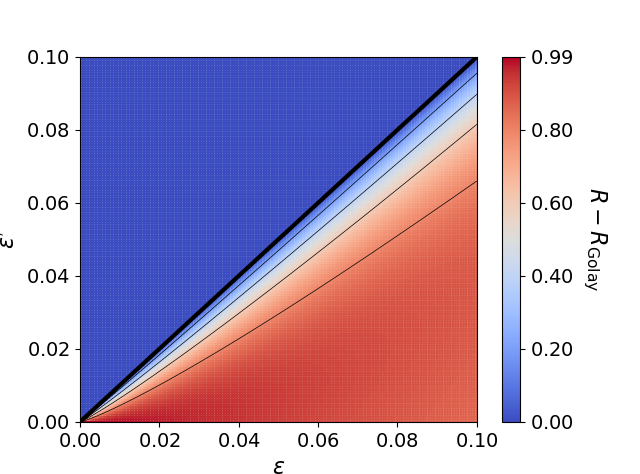
\includegraphics[scale=0.5]{figs/prakash_compare.png}
    \caption{\textbf{Comparison with ternary Golay distillation rate.}
    Our bound is not violated but gets close to saturated for some noise levels.
    The thick diagonal line indicates where $\epsilon' = \epsilon$.
    }
    \label{fig:prakash_compare}
\end{figure}

We can also rewrite the expression as 
\begin{equation}
	\epsilon_{\rm{Golay}}(\epsilon', n) \approx \frac{1}{\alpha}(\alpha\epsilon')^{n^{-\xi}},
\end{equation}
and compare with the numerically optimal error bounds provided by majorisation as shown in~\cref{fig:prakash_compare_errors}
\begin{figure}[h]
    \centering
    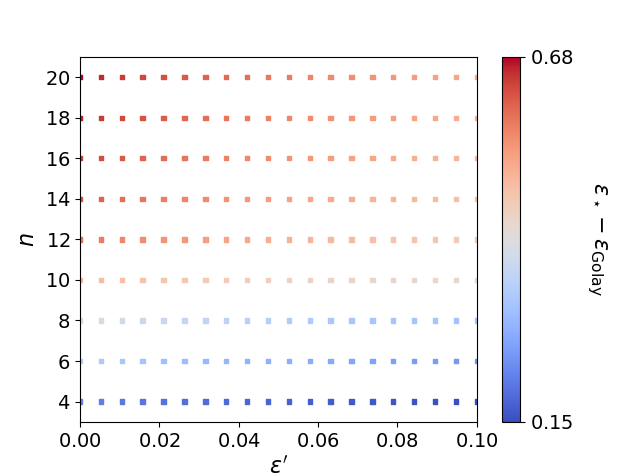
\includegraphics[scale=0.5]{figs/prakash_compare_errors.png}
    \caption{\textbf{Comparison with ternary Golay output error rate.}
    Our bound is not violated but achieves a maximum saturation of $\epsilon_\star - \epsilon_{\rm{Golay}} = 0.147$.
    }
    \label{fig:prakash_compare_errors}
\end{figure}

A recent distillation bound was introduced in~\cite{Seddon2020}, where they show that for the deterministic conversion of $n$ copies of a qubit state $\rho$ to a target pure magic state $\ket{\psi}$, the following bound on the distillation rate holds,
\begin{equation}\label{eq:seddon}
	\frac{n'}{n} \leq \frac{\log{\Lambda^+(\rho)}}{\log{F(\psi)^{-1}}},
\end{equation}
where $\Lambda^+(\rho)$ is the generalised robustness of state $\rho$, calculable via a costly SDP and $F(\psi)$ denotes the stabiliser fidelity of state $\ket{\psi}$.
They demonstrate the performance of their bound by considering the purification process of the qubit magic state $\ket{H}$, with their figure replicated in~\cref{fig:seddon}. 
For high initial noise level ($\epsilon = 0.25$), their bound dictates that $R = 1/150$, which is pretty good.
\begin{figure}[h]
    \centering
    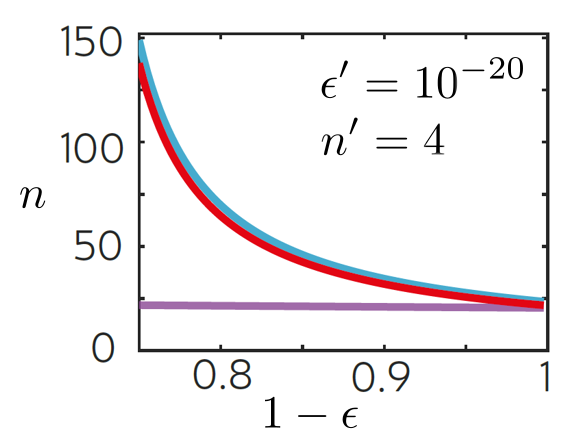
\includegraphics[scale=0.3]{figs/seddon.png}
    \caption{\textbf{Comparison of Seddon \textit{et al.}'s bound~\cite{Seddon2020} in~\cref{eq:seddon} with a generic resource bound in~\cite{Fang2020}.}
    The process they consider is purifying $n$ copies of $(1-\epsilon)\ketbra{H} + \epsilon/3 \id$ to $n'$ copies of $(1-\epsilon')\ketbra{H} + \epsilon'/3 \id$.
    Their bound (red and blue) is pretty good compared with the generic (violet) bound.
    Not sure why it looks like their bound gives $n\rightarrow 25$ as $1-\epsilon \rightarrow 1$.
    }
    \label{fig:seddon}
\end{figure}

Similar concrete rates have been studied for qudits in two occasions:
First, the mana bound, which we have demonstrated in~\cref{fig:distill_bounds}.
Secondly, Wang \textit{et al.}'s max-thauma bound~\cite{Wang2020}, which as far as I can tell, is less tight than mana (?).
It is defined via an SDP, but we can use its properties (super-additivity and zero at free states) to readily get a bound on noisy Strange states,
\begin{equation}
	\theta_{\rm{max}}(\rho_{\rm{S}}(\epsilon)) \geq (1-\epsilon) \ketbra{\rm{S}} + \epsilon \frac{1}{3}\id = (1-\epsilon) \theta_{\rm{max}}(\rho_{\rm{S}}(0)).
\end{equation}
Their bound simply states that any deterministic single-copy distillation process $\rho^{\otimes n} \longrightarrow \tau$ requires an initial number of copies $n \geq \theta_{\rm{max}}(\tau) / \theta_{\rm{max}}(\rho)$.
Therefore, the rate of our pure Strange state distillation process~\cref{eq:sudist} can only get as tight as
\begin{equation}
	R = 1/n = \frac{\theta_{\rm{max}}(\rho_{\rm{S}}(\epsilon))}{\theta_{\rm{max}}(\rho_{\rm{S}}(0))} \leq 1-\epsilon,
\end{equation}
which is less tight than mana as could be readily observed if plotted in~\cref{fig:distill_bounds}.

An $n$-copy state $\rho^n$ has \emph{error rate} $\delta$ iff $\rho$ has an overlap of at least $1-\delta$ with magic state $\ket{\rm{S}}$,
\begin{equation}
	\bra{\rm{S}}\rho\ket{\rm{S}} \geq 1-\delta.
\end{equation}
The $\epsilon$-noisy Strange state $\rho_{\rm{S}}(\epsilon)^{\otimes n}$ has error rate $\delta = \frac{2}{3}\epsilon$.
A general state of $n$ qutrits with error rate $\delta$ can be converted to the form $\rho_{\rm{S}}(\epsilon_0)^{\otimes n}$ for some noise level $\epsilon$ not necessarily equal to $\delta$.

Given an $[[m,k,d]]$ error correcting code, a distillation protocol that achieves the process in~\cref{eq:test} requires that the following bound holds,
\begin{align}
	\frac{n}{n'} = O(\log^\gamma{(1/\epsilon')}),\ \gamma = \log_d{\left(\frac{m}{k}\right)}
\end{align}

In~\cite{Bravyi2012,Hastings2018}, the asymptotic rate $O(\log^\gamma{(1/\epsilon')})$ is called the \emph{distillation cost}, and in~\cite{cit:bravyi,Krishna2019} the parameter $\gamma$ is called the \emph{overhead}.

There are many distillation protocols in the literature, e.g.~\cite{Bravyi2012,Hastings2018}, that involve a specific value of $\gamma$ and convert a specific number of copies $n$ of input states to $n'=1$ output state \nick{what about $\epsilon$?}.
They should all satisfy
\begin{equation}\label{eq:rate_cost}
	\frac{1}{R(\epsilon, \epsilon', \beta)} \leq \frac{n}{n'} = O(\log^\gamma{(1/\epsilon')}).
\end{equation}
Therefore, given process parameters $n, n', \epsilon, \epsilon'$, we can scan through the stabiliser states to find a range of $\beta$ for which inequality~\cref{eq:rate_cost} is valid.
In principle, the higher the value of parameter $\gamma$, the lower the output error rate $\epsilon'$ can be while~\cref{eq:rate_cost} is still true.
In~\cite{Hastings2018} \nick{CITE MORE}, they report a value of $\gamma = 0.6779\dots$, while in~\cite{Krishna2019}, they report a scaling $\gamma = O(1/\log{d})$ with respect to the system's odd prime dimension $d$.
The latter tends to 0 asymptotically.

We can rephrase this result, saying that any distillation protocol in the $\gamma_\beta$-fragment with an $n$-copy input and $n'$-copy, $\epsilon'$-noisy desired output, must have input noise level 
\begin{equation}
	\epsilon \leq  E\left(\frac{n'}{n}, \epsilon', \beta \right)
\end{equation}
for some error bound $E$ related to $R$.

Furthermore, in~\cite{cit:bravyi,cit:prakash}, two different distillation protocols are proposed with output error rate scalings of the form 
\begin{equation}
	\epsilon' \propto (\alpha \epsilon)^{n^\xi},
\end{equation}
where $\alpha$ is some constant, $\xi = 1/\log_3{15} \approx 0.4$ in~\cite{cit:bravyi} for qubit codes and $\xi = 1/\log_3{19008} \approx 0.1$ for qutrit codes.
They also report a certain input threshold error rate $\epsilon_\star$ above which distillation is not possible.
A first requirement is that $\epsilon_\star \leq E(n'/n, \epsilon', \beta)$, but we can also again find a range of $\beta$ for which the inequality
\begin{align}
	\epsilon &\leq E\left(\frac{n'}{n}, \epsilon'(\epsilon), \beta \right) \\
	\epsilon' &\sim O\left((n\epsilon)^d\right)
\end{align}
holds, given some distillation rate $n'/n$ and input error rate $\epsilon$.

\null\newpage
%%%%%%%%%%%%%%%%%%%%%%%%%%%%%%%%%%%%%%%%

\section{Random info}
\begin{figure}[h]
    \centering
    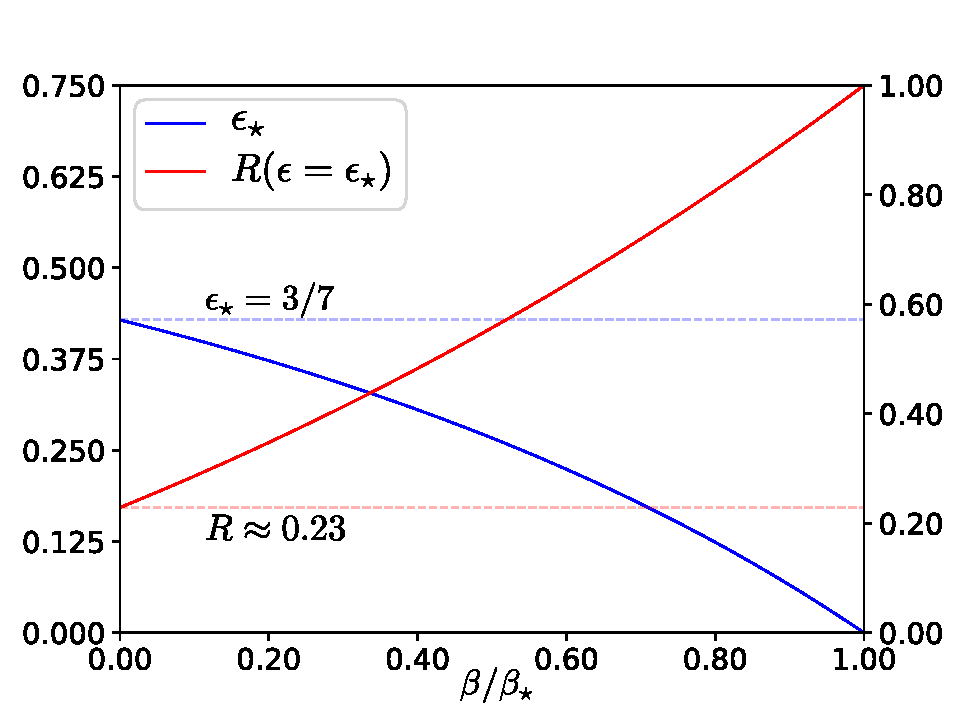
\includegraphics[scale=0.5]{figs/noise_threshold.pdf}
    \caption{\textbf{Noise threshold $\epsilon_\star$ and rate $R(\beta, \epsilon_\star)$ versus $\beta$.}
    At $\beta = 0$ and threshold noise level $\epsilon = \epsilon_\star = 3/7$, the rate is $R(0, \epsilon_\star) = \frac{\ln{(9/7)}}{\ln{3}} \approx 0.23$.
    }
    \label{fig:noise_threshold}
\end{figure}

We generalise the analysis of unital fragments into any circuit with thermalisation noise parametrised by the temperature $\beta^{-1}$.
In~\cref{fig:thermal_distill}, we examine the majorisation bound for the same purification process of~\cref{eq:sdist} with $\epsilon' = 0.05$.
The curves plotted suggest that there exists a fragment $\O_{\gamma_{\beta_{\rm{max}}}}$ which allows for a highest noise threshold at any given number of copies of the initial state.
Adding more copies results in a lower optimal temperature $\beta^{-1}$.

\begin{figure}[h]
    \centering
    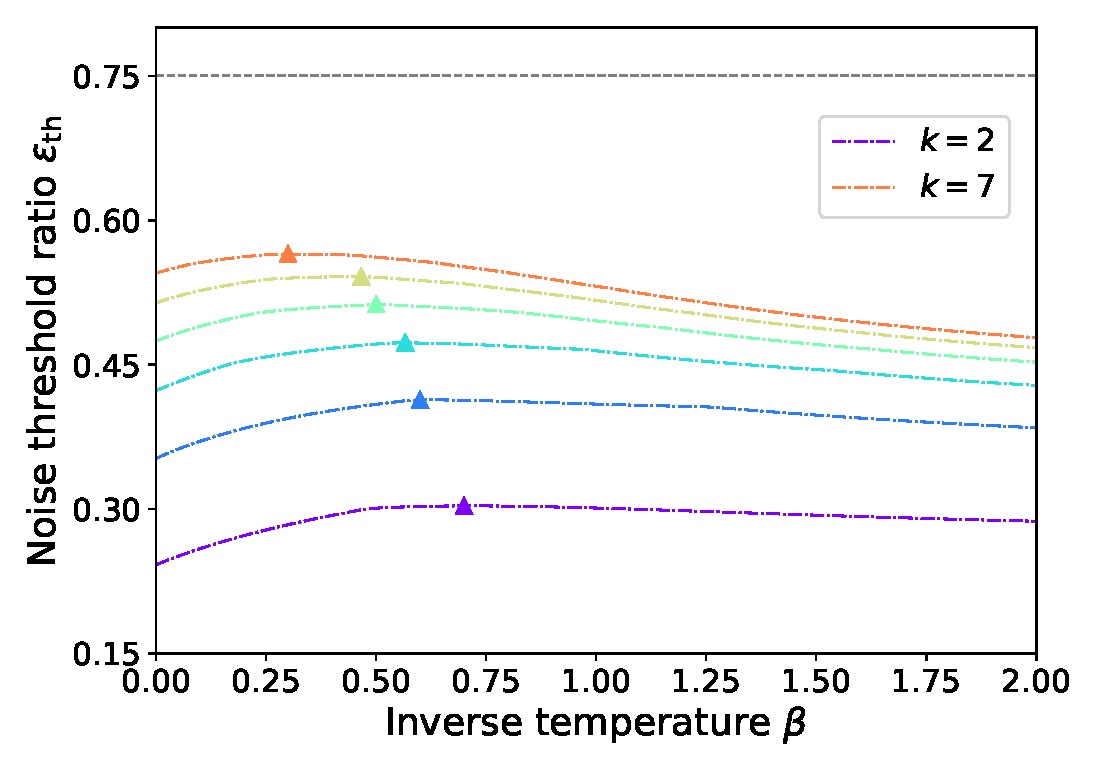
\includegraphics[scale=0.5]{figs/thermal_distill.pdf}
    \caption{\textbf{Threshold dependence on temperature in thermal fragments.} Lorenz curve ratios for the Strange state purifying process in~\cref{eq:sdist} with $\epsilon' = 0.05$.
    The peaks of each curve indicate the optimal temperature $\beta_{\rm{max}}^{-1}$ that allows for the highest noise threshold at every given number of initial state copies $k$.
    The line $\epsilon = \frac{3}{4}$ indicates the threshold noise beyond which the Strange state no longer contains negativities.
    }
    \label{fig:thermal_distill}
\end{figure}

\null\newpage
%%%%%%%%%%%%%%%%%%%%%%%%%%%%%%%%%%%%%%%%

\section{Phi bounds}

\begin{figure}[t]
    \centering
    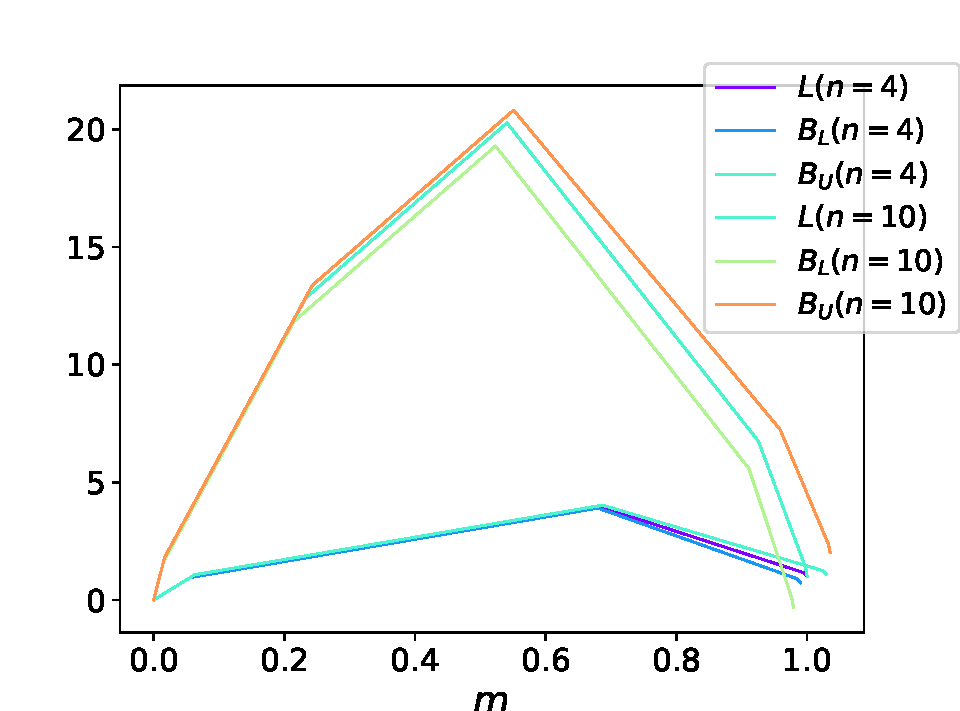
\includegraphics[scale=0.4]{figs/lc_bounds.pdf}
    \caption{\textbf{Lorenz curves and bounding curves.} 
    The figure explores the distillation process of a 10-copy $0.25$--noisy Strange state to a 4-copy $0.05$--noisy Strange state in the unital fragment.
    Clearly, by looking at the Lorenz curves, the distillation process is possible.
    However the bounding curves, derived in~\cref{lem:bounds_strict}, intersect at the end, suggesting that the process is not necessarily possible.
    }
    \label{fig:lc_bounds}
\end{figure}

The experiment is described by binomial statistics and we define the left tail of the cumulative binomial distribution,
\begin{equation}\label{eq:phil}
	\Phi_\ell(m; n, p) \coloneqq \sum\limits_{j=0}^m \binom{n}{j} p^j (1-p)^{n-j},
\end{equation}
where $m\in [0,n]$. 

The symmetry between the left tail of a $p$--coin distribution and the right tail of a $(1-p)$--coin distribution dictates that
\begin{align}\label{eq:phi_reverse}
	\Phi_\ell(m; n, p) + \Phi_\ell(n-m-1; n, 1-p) &= 1,\ m\in [0,n-1],
\end{align}
Entropic bounds on $\Phi_\ell$~\cite{cit:ash}.
\begin{lemma}\label{lem:phil_bounds}
	Given fixed $n>0$ and $p$, $\Phi_\ell$ satisfies the following bounds:
	\begin{align*}
		\begin{split}
		&\text{1. } \Phi_\ell(m; n, p) \geq \left[ 8m\left(1-\frac{m}{n}\right) \right]^{-\frac{1}{2}} 2^{-n \ent{p}{q}},\ m\in [1,n-1] \\
		&\text{2. } \Phi_\ell(m; n, p) \leq 2^{-n\ent{p}{q}},\ m\in [0,np] \\
		&\text{3. } \Phi_\ell(m; n, p) \leq 1 - \left[ 8(m+1)\left(1-\frac{m+1}{n}\right) \right]^{-\frac{1}{2}} 2^{-n\ent{\frac{m+1}{n}}{p}}, \\
		&\hspace{14pt} m\in [0,n-2]
		\end{split}
		\\
		&\text{4. } \Phi_\ell(m; n, p) \geq 1 - 2^{-n\ent{\frac{m+1}{n}}{p}},\ m\in [np+1,n-2]
	\end{align*}
\end{lemma}
\begin{proof}
	\nick{cite proof}
\end{proof}
Loose bounds follow
\begin{lemma}\label{lem:bounds_loose}
	Given fixed $n>0$ and $p$, $\Phi$ satisfies the following bounds:
	\begin{align*}
		\begin{split}
		&\text{1. } \Phi_{\pm}(m; n, p) \geq \left[ 8m\left(1-\frac{m}{n}\right) \right]^{-\frac{1}{2}} 2^{-n\ent{p}{q}},\ m\in [1,n-1] \\
		&\text{2. } \Phi_{\pm}(m; n, p) \leq 2^{-n\ent{p}{q}},\ m\in [0,np] \\
		&\text{3. } \Phi_{\pm}(m; n, p) \leq 1 - \left[ 8(m+1)\left(1-\frac{m+1}{n}\right) \right]^{-\frac{1}{2}} 2^{-n\ent{\frac{m+1}{n}}{p}}, \\
		&\hspace{14pt} m\in [0,n-2]
		\end{split}
	\end{align*}
\end{lemma}
\begin{proof}
	\nick{paste proof}
\end{proof}

We can therefore use~\cref{lem:bounds_loose,lem:bounds_strict} to bound the standard Lorenz curves.



\subsection{Strange state MSD in the unital fragment}\label{app:lc_compare}

Consider the Strange state MSD process in the unital fragment,
\begin{equation}\label{eq:su_conversion}
    \rho_{\rm{S}}(n', \epsilon, 0) \xrightarrow{\mathcal{O}_{\id/3}} \rho_{\rm{S}}(n', \epsilon', n-n').
\end{equation}
We denote input state indices without a prime and target state indices with a prime,
\begin{align}
    I(i,j,k=1) &= j + \sum_{\ell=0}^{i-1} m_{\ell}(n, \epsilon), \\
    I'(i',j',k') &= k' + \left[ (j'-1) + \sum_{\ell=0}^{i'-1} m_{\ell}(n', \epsilon') \right]9^{n-n'}.
\end{align}

Pointwise Lorenz curve comparison requires $x_{I} = x_{I'}$, so the question is: 
\begin{center}
\emph{Given a triplet $(i',j',k')$, what is the tuple $(i,j)$ such that $I(i,j) = I'(i',j',k')$?}
\end{center}

According to~\cref{thm:elbows} which is proved in~\cref{app:lc_constraints}, for standard Lorenz curves, we need to match indices at the target state elbows, so the requirement on the indices is finding a tuple $(i, j)$, such that for a given $i' = 0,\dots,n'$,
\begin{equation}
	j + \sum_{\ell=0}^{i-1} m_{\ell}(n, \epsilon) = \sum_{\ell=0}^{i'} m_{\ell}(n', \epsilon').
\end{equation}

As a basic example, consider the process 
\begin{equation}
\rho_{\rm{S}}(\epsilon)^{\otimes 4} \xrightarrow{\mathcal{O}_{\id/3}} \rho_{\rm{S}}(\epsilon')^{\otimes 2} \otimes \left( \frac{1}{3}\id \right)^{\otimes 2}.
\end{equation}
We want to check which Lorenz curve is higher at the first elbows of the target state, i.e. we want to verify or reject the first inequality below:
\begin{equation}
	L_{I(i,j)} \geq L'_{I'(0, 1, 81)}
\end{equation}
where the first multiplicity of the target state is $m_0 = 1$.
The multiplicities of the initial state are $(1, 384, 4096)$.

The challenge is to find $i,j$ such that $i(i,j) = i'(0,1,81)$.
\nick{By trial and error}, we find that $(i,j) = (1, 80)$.
Now we can use~\cref{eq:lcsu_lcoord} to directly calculate
\begin{align*}
	L'_{i'(0,1,81)} &= L'_0 = \left( \frac{5}{3} - \frac{8}{9}\epsilon\ \right)^2 \Phi_+\left(0;2,4\frac{3-\epsilon}{15-8\epsilon}\right), \\
	L_{i(1, 80)} &= \left(1-\frac{80}{384} \right) L_0 + \frac{80}{384} L_1 \\
	\begin{split}
	&= \left( \frac{5}{3} - \frac{8}{9}\epsilon\ \right)^4 \bigg[ \frac{19}{24} \Phi_+\left(0;4,4\frac{3-\epsilon}{15-8\epsilon}\right) \\ 
	&\qquad + \frac{5}{24}\Phi_+\left(2;4,4\frac{3-\epsilon}{15-8\epsilon}\right) \bigg],
	\end{split}
\end{align*}
and then compare them.

With the help of this lemma, we directly arrive at 
\begin{theorem}\label{thm:bounds_strict}
	Given fixed positive integer $n$ and probability $p$, $\Phi_+, \Phi_-$ satisfy the following bounds:
	\begin{align*}
		\begin{split}
		&\text{1. } \Phi_+(m; n, p) \geq \sum\limits_{\ell=0}^{m/2}\left[ 16\ell\left(1-\frac{2\ell}{n}\right) \right]^{-\frac{1}{2}} 2^{-n\ent{\frac{2\ell}{n}}{p}}, \\
		&\hspace{14pt} \text{for all even } m\in [2,n] \\
		&\text{2. } \Phi_+(m; n, p) \leq \sum\limits_{\ell=0}^{m/2}\left[ 4\pi\ell\left(1-\frac{2\ell}{n}\right) \right]^{-\frac{1}{2}} 2^{-n\ent{\frac{2\ell}{n}}{p}}, \\
		&\hspace{14pt} \text{for all even } a\in [2,n] \\
		&\text{3. } \Phi_-(m; n, p) \geq \sum\limits_{\ell=1}^{(m-1)/2}\left[ 16(\ell+1)\left(1-\frac{2\ell+1}{n}\right) \right]^{-\frac{1}{2}} \times \\
		&\hspace{14pt} \times 2^{-n\ent{\frac{2\ell+1}{n}}{p}},\ \text{for all odd }a\in [1,n] \\
		&\text{4. } \Phi_-(m; n, p) \leq \sum\limits_{\ell=1}^{(m-1)/2}\left[ 4\pi(\ell+1)\left(1-\frac{2\ell+1}{n}\right) \right]^{-\frac{1}{2}} \times \\
		&\hspace{14pt} \times 2^{-n\ent{\frac{2\ell+1}{n}}{p}},\ \text{for all odd } a\in [1,n]
		\end{split}
	\end{align*}
\end{theorem}
\begin{proof}
	All four statements follow from application of~\cref{lem:comb_bounds} on the combinatorial coefficient and the defintion of relative entropy given in~\cref{eq:ent_rel}
\end{proof}

\null\newpage
%%%%%%%%%%%%%%%%%%%%%%%%%%%%%%%%%%%%%%%%

\section{Area monotone}\label{app:areamono}

\nick{I don't believe in the area monotone - should we keep?}

\begin{figure}[h]%
    \centering
    \subfigure[][]{%
    \label{fig:test1}%
    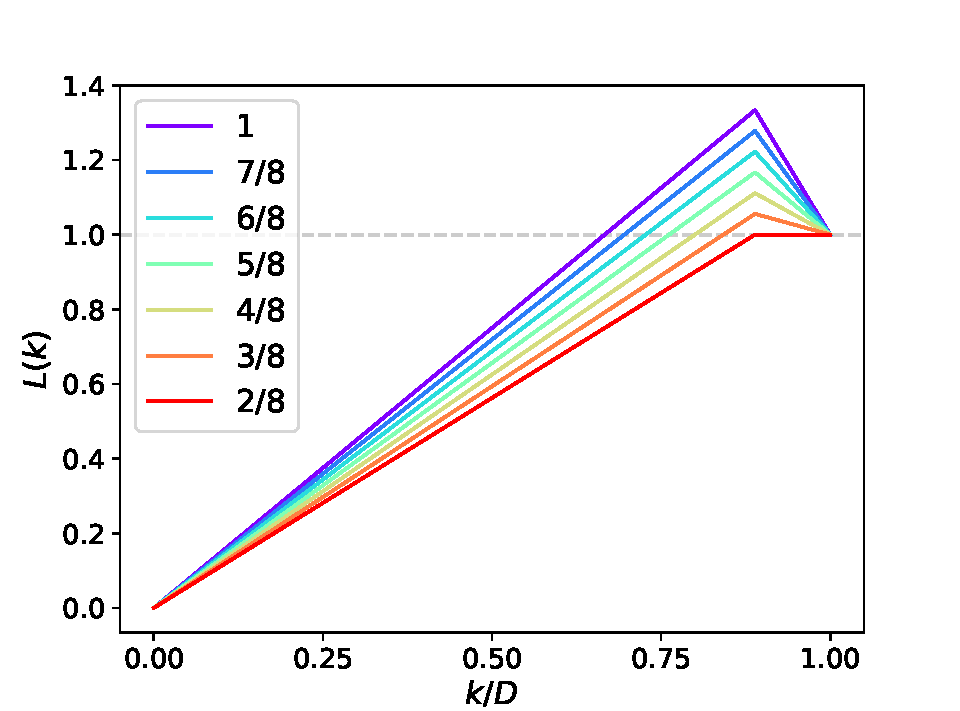
\includegraphics[height=3cm]{figs/negmasking_rho_strange_lc.pdf}
    %\caption{Maximally mixed state $\frac{1}{3}\id$}%
    }\hspace{8pt}%
    \subfigure[][]{%
    \label{fig:test2}%
    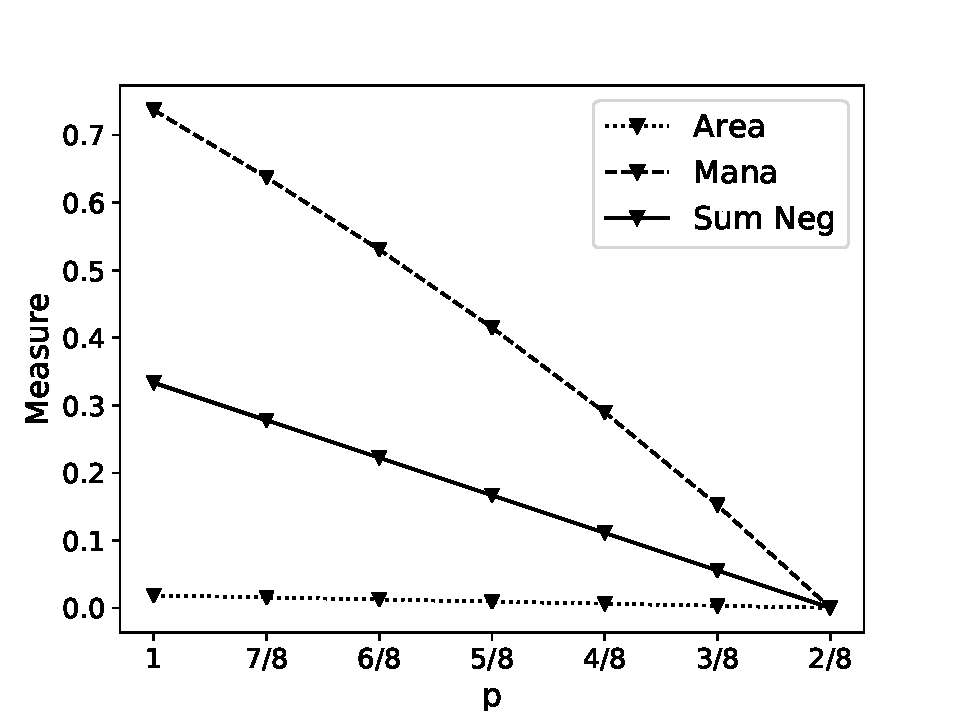
\includegraphics[height=3cm]{figs/negmasking_rho_strange_meas.pdf}
    %\caption{Zero state $\ketbra{0}{0}$}%
    }
    \caption{\subref{fig:test1} Lorenz curve of $p\ketbra{\rm{S}} + (1-p) \frac{1}{d}\id$ for $p$ given in the legend.\subref{fig:test2} Different measures for the states on the left. \\
    \nick{can replace~\cref{fig:lctoy} with a more informative version of this figure}
    }%
    \label{fig:test}
\end{figure}

Let $L_{>1}$ be the set of points on the Lorenz curve $\lc{\rho}{\sigma}(k)$ that lie above $1$ of state $\rho$ in the $\sigma$--fragment. 
If $\rho$ is a free state, $L_{>1}$ is empty and $\A_\sigma(\rho) = 0$. 
Otherwise, $\A_\sigma(\rho) > 0$ and it can be calculated exactly using the trapezium rule or the shoelace formula. 
Let $k$ be the index of the first point $\left(x_k, \lc{\rho}{\sigma}(k)\right)$ lying above $1$. 
Then $L_\rho(k)$ crosses $1$ at
\begin{equation}
	x_{\rm{int}} = x_k - \frac{x_k - x_{k-1}}{\lc{\rho}{\sigma}(k) - \lc{\rho}{\sigma}(k-1)}\lc{\rho}{\sigma}(k),\vspace{10pt}
\end{equation}
as well as at $\left(x_d, \lc{\rho}{\sigma}(d)\right) = (1,1)$

Now we can define
\begin{equation}
L_{>1}^+ = \{ (x_i, y_i) \}_{0 \leq i \leq n}
\end{equation}
such that it contains the initial point of intersection $(x_0, y_0) \equiv (x_{n+1}, y_{n+1}) \coloneqq (x_{\rm{int}}, 1)$, all points $(x_i, y_i)$, labelled by $i=1,\dots,n-1$ that lie above $y=1$ contained in $L_{>1}$ and finally the second point of intersection $(x_n, y_n) = (1,1)$.
Then, 
\begin{equation}
	\A_\sigma(\rho) = \frac{1}{2} \sum\limits_{i=0}^n (x_{i+1} y_i - x_i y_{i+1}).
\end{equation}

We note that single-copy Lorenz curves are additive in noise, 
\begin{equation}
	\lc{(1-\epsilon)\rho + \epsilon\sigma}{\sigma} = (1-\epsilon)\lc{\rho}{\sigma} + \epsilon\lc{\sigma}{\sigma},
\end{equation}
for any $\sigma, \rho$.
This is not true for higher number of copies.

\nick{In particular}, it can be used in the discussion of standard Lorenz curves to set the necessary constraints,
\begin{align}
L\left(x_{I'(0, m'_{0}, 9^{n-n'})}\right) &\geq L\left(x_{I'(0, m'_{0}, 9^{n-n'})}\right), \nonumber\\
L\left(x_{I'(1, m'_{1}, 9^{n-n'})}\right) &\geq L\left(x_{I'(1, m'_{1}, 9^{n-n'})}\right), \nonumber\\
&\vdotswithin{=} \nonumber\\
L\left(x_{I'(n', m'_{r}, 9^{n-n'})}\right) &\geq L\left(x_{I'(n', m'_{n'}, 9^{n-n'})}\right), \nonumber
\end{align}
where $x_{I'(0, m'_{0}, 9^{n - n'})}, x_{I'(1, m'_{1}, 9^{n - n'})}, \dots, x_{I'(n', m'_{n'}, 9^{n - n'})} \in T$ are the locations of the elbows of $\lc{\rho_{\rm{S}}(\epsilon')^{\otimes n'}}{\frac{1}{d}\id}$ (excluding $0$ and $1$).

\null\newpage
%%%%%%%%%%%%%%%%%%%%%%%%%%%%%%%%%%%%%%%%

\section{Stabilizer proof details}

Whether we are dealing with $\rm{(C1)}$ or $\rm{(C2)}$ depends on the physical parameters $\beta$ and $\epsilon$ as follows:
\begin{itemize}
	\item $\beta = 0$. Then, $\epsilon_{\star} = 3/7$ and $\rm{(C1)}$ holds for all noise levels $\epsilon$.
	This is the unital fragment.
	\item $0 < \beta \leq \beta_{\star}$. Then, $0 \leq \epsilon_{\star} < 3/7$ and $\rm{(C1)}$ holds for $\epsilon \leq \epsilon_{\star}$, while $\rm{(C2)}$ holds for $\epsilon \geq \epsilon_{\star}$.
	\item $\beta > \beta_{\star}$. Then, $ \epsilon_{\star} = 0$ and $\rm{(C2)}$ holds for all $\epsilon$.
\end{itemize}

Consider pure Strange state distillation at high temperatures, $\beta \leq \beta_{\star}$.
Depending on the noise level of the initial state, we have either a $\rm{(C1)} \rightarrow \rm{(C1)}$ or a $\rm{(C2)} \rightarrow \rm{(C1)}$ scenario.

At every $\beta > 0$, the rates indicate a transition at $\epsilon_{\star}$.
As $\beta$ increases, the rate becomes stricter.
At the high temperature limit, $\beta \rightarrow 0$, we get $\beta F_\beta \rightarrow -\ln{3}$, and we retrieve the unital fragment bound,
\begin{equation}
	R(\beta) \xrightarrow{\beta \rightarrow 0} \frac{\ln{(3-4\epsilon)}}{\ln{3}}.
\end{equation}

Consider pure Strange state distillation at low temperatures, $\beta \rightarrow \infty$.
Independently of the noise level of the initial state, we have a $\rm{(C2)} \rightarrow \rm{(C2)}$ scenario.

As $\beta$ increases, the rate becomes looser.
At the zero temperature limit, $F_\beta$ tends to zero, so $R(\epsilon, \beta) \xrightarrow{\beta \rightarrow \infty} 1$.

\subsection{First elbow location}
\label{app:first_elb_loc}
Consider a magic state interconversion in a stabilizer $\sigma$--fragment, as in~\cref{eq:stdist}, where we remind that $n \geq n'$ and we denote by $(x_0, L_0)$ and $(x'_0, L'_0)$ the first elbow coordinates of the initial and target states respectively.

Here, we show that $x_0 \leq x'_0$ for any of the three scenarios outlined in the proof of our main theorem in~\cref{sec:stab}.\\

$\rm{(C1)} \rightarrow \rm{(C1)}$.
We know from statistical physics that $e^{-\beta E_0} / \Z_\beta \leq 1$, so
	\begin{align*}
		x_0 &= \left(\dfrac{e^{-\beta E_0}}{3\Z_\beta}\right)^n = \left(\dfrac{e^{-\beta E_0}}{3\Z_\beta}\right)^{n-n'} \left(\dfrac{e^{-\beta E_0}}{3\Z_\beta}\right)^{n'} \\
		&< \left(\dfrac{e^{-\beta E_0}}{3\Z_\beta}\right)^{n'} = x_0'		
	\end{align*}

$\rm{(C2)} \rightarrow \rm{(C1)}$.
We now use the slightly altered inequality $e^{-\beta E_{\rm{max}}} / \Z_\beta \leq 1$ to proceed,
	\begin{align*}
		x_0 &= \left(\dfrac{e^{-\beta E_{\rm{max}}}}{\Z_\beta}\right)^n = \dfrac{e^{-\beta(n E_{\rm{max}} - n' E_0)}}{\Z_\beta^{n-n'}} \left(\dfrac{e^{-\beta E_0}}{3\Z_\beta}\right)^{n'} \\
		&\leq \dfrac{e^{-\beta(n E_{\rm{max}} - n' E_0)}}{e^{-\beta (n-n') E_{\rm{max}}}} \left(\dfrac{e^{-\beta E_0}}{3\Z_\beta}\right)^{n'} \\
		&= e^{-\beta n' (E_{\rm{max}} - E_0)} \left(\dfrac{e^{-\beta E_0}}{3\Z_\beta}\right)^{n'} \\
		&\leq \left(\dfrac{e^{-\beta E_0}}{3\Z_\beta}\right)^{n'} = x_0'.
	\end{align*}

$\rm{(C2)} \rightarrow \rm{(C2)}$.
Similarly in this scenario,
	\begin{align*}
		x_0 &= \left(\dfrac{e^{-\beta E_{\rm{max}}}}{\Z_\beta}\right)^n = \left(\dfrac{e^{-\beta E_{\rm{max}}}}{\Z_\beta}\right)^{n-n'} \left(\dfrac{e^{-\beta E_{\rm{max}}}}{\Z_\beta}\right)^{n'} \\
		&\leq \left(\dfrac{e^{-\beta E_{\rm{max}}}}{\Z_\beta}\right)^{n'} = x_0'	
	\end{align*}
	
\subsection{Deriving distillation bounds from the last elbow}
\label{sec:last_elb}

\nick{RESTRUCTURE}

To find the coordinates of the \textbf{last} elbow $(x_E, L_E)$, where $E$ is the number of elbows, we need to evaluate the minimum rescaled component,
\begin{align}
	&\bmw(\rho_{\rm{S}} | \sigma)_{\rm{min}} \coloneqq (3\Z)^{n}\times \nonumber\\
	&\min\limits_{i,j,k}\Big\{ (-v)^{n-\alpha} u^{\alpha} e^{\beta (n-\alpha)E_0} e^{\beta ( i E_0 + j E_1 + k E_2 )} \Big\}, \label{eq:min_slope}
\end{align}
where $0 \leq i,j,k \leq n$ and $\alpha \coloneqq i+j+k \leq n$.
Notice that for $0 \leq \epsilon \leq 3/7$, we have $v \geq u$. 
We need the sum $\alpha = i+j+k$ to be odd for the expression to be negative.

Given an odd value for the sum $\alpha$, the term $v^{n-\alpha} u^{\alpha} e^{-\beta (n-\alpha)E_0}$ is fixed (and negative), so the expression is minimised by setting the coefficient of the highest energy $E_{\rm{max}}$ equal to $\alpha$.
Hence, we have
\begin{align}
	&\bmw(\rho_{\rm{S}} | \sigma)_{\rm{min}} = \nonumber\\
	&-(3\Z)^{n} v^n e^{n\beta E_0}\max\limits_{\substack{\alpha = 1,3, \\ \dots,n-1}}{\Big\{ \left( \frac{u}{v} e^{\beta (E_{\rm{max}} - E_0)} \right)^{\alpha} \Big\}}.
\end{align}
If the expression $\frac{u}{v} e^{\beta (E_{\rm{max}} - E_0)}$ is less than $1$ then the minimum occurs at $\alpha=1$, otherwise it occurs at $\alpha = n-1$.

The minimum rescaled component can then be expressed as
\begin{equation}
\bmw(\rho_{\rm{S}} | \sigma)_{\rm{min}} =
	\begin{cases}
		-(3\Z)^{n} v^{n-1} u e^{\beta [(n-1)E_0 + E_{\rm{max}}]}, &\epsilon \leq \epsilon_{\star},\ \hspace{3pt}\rm{(C1)}	\\
		-(3\Z)^{n} v u^{n-1} e^{\beta [E_0 + (n-1)E_{\rm{max}}]}, &\epsilon > \epsilon_{\star}.\ \hspace{5pt}\rm{(C2)} 
	\end{cases}
\end{equation}
Case $\rm{(C1)}$ can correspond to $(i,j,k) = (1,0,0)$ if $E_{\rm{max}} = E_0$, when the multiplicity is $m_{100} = 2n$ and the corresponding Wigner components are $\bmw(\rho_{\rm{S}})_{100}, \bmw(\sigma)_{100}$ or it can correspond to $(i,j,k) = (0,1,0)$ ($(i,j,k) = (0,0,1)$), if $E_{\rm{max}} = E_1$ ($E_{\rm{max}} = E_2$), when the multiplicity is $m_{010} = 3n$ ($m_{001} = 3n$) and the corresponding Wigner components are $\bmw(\rho_{\rm{S}})_{010}, \bmw(\sigma)_{010}$ ($\bmw(\rho_{\rm{S}})_{001}, \bmw(\sigma)_{001}$).
Case $\rm{(C2)}$ corresponds to $(i,j,k) = (0,n-1,0)$ ($(i,j,k) = (0,0,n-1)$)
if we have $E_{\rm{max}} = E_1$ ($E_{\rm{max}} = E_2$), when the multiplicity is $m_{0,n-1,0} = 3^{n-1}n$ ($m_{0,0,n-1} = 3^{n-1}n$) and the corresponding Wigner components are $\bmw(\rho_{\rm{S}})_{0,n-1,0}, \bmw(\sigma)_{0,n-1,0}$ ($\bmw(\rho_{\rm{S}})_{0,0,n-1}, \bmw(\sigma)_{0,0,n-1}$).

The last elbow coordinates can finally be derived by sutracting the appropriate rescaled component from 1, $(x_E, L_E) =$
\begin{equation}\label{eq:last_elb_coords}
	\begin{cases}
		&\left( 1-\dfrac{2n}{(3\Z_\beta)^n}e^{-\beta [(n-1)E_0 + E_{\rm{max}}]},\ 1 + 2n v^{n-1} u \right), \vspace{5pt}\\
		&\hspace{5pt} \text{if } E_{\rm{max}} = E_0, \hspace{51pt}\rm{(C1a)} \vspace{10pt}\\
		&\left( 1-\dfrac{3n}{(3\Z_\beta)^n}e^{-\beta [(n-1)E_0 + E_{\rm{max}}]},\ 1 + 3n v^{n-1} u \right), \vspace{5pt}\\
		&\hspace{5pt} \text{if } E_{\rm{max}} > E_0, \epsilon \leq \epsilon_{\star}, \hspace{20pt}\rm{(C1b)} \vspace{10pt}\\
		&\left( 1-\dfrac{n}{3\Z_\beta^n}e^{-\beta [E_0 + (n-1)E_{\rm{max}}]},\ 1 + 3^{n-1}n v u^{n-1} \right), \vspace{5pt}\\
		&\hspace{5pt} \text{if } E_{\rm{max}} > E_0, \epsilon \geq \epsilon_{\star}. \hspace{22pt}\rm{(C2)}
	\end{cases}
\end{equation}

Assuming that $E_{\rm{max}} > E_0$ for clarity, we have the same three scenarios as in the case of the first elbow bound:
\begin{enumerate}
	\item $\rm{(C1)} \rightarrow \rm{(C1)}$ if $\beta < \beta_{\star}$ and $\epsilon' < \epsilon  \leq \epsilon_{\star}$.
	\item $\rm{(C2)} \rightarrow \rm{(C1)}$ if $\beta < \beta_{\star}$ and $\epsilon' \leq \epsilon_{\star} < \epsilon$.
	\item $\rm{(C2)} \rightarrow \rm{(C2)}$ if $\beta < \beta_{\star}$ and $\epsilon_{\star} \leq \epsilon' < \epsilon$ or $\beta \geq \beta_{\star}$.
\end{enumerate}
Now using last elbow constraint, derived in~\cref{app:elb_constraints}, we can calculate new distillation bounds.
The last elbow bounds can be rephrased in terms of the first elbow bound, leading to $R_{\rm{last-elb}} - R_{\rm{first-elb}} = $
\begin{equation}\label{eq:last_elb_coords}
	\begin{cases}
		\dfrac{1}{n} \dfrac{\log{\frac{u(\epsilon)v(\epsilon')}{u(\epsilon')v(\epsilon)}}}{\ln{\big( 1-\frac{4}{3}\epsilon' \big)} + \beta (E_0 - F(\beta))},\ &\rm{(C1)} \rightarrow \rm{(C1)}, \vspace{10pt}\\
		\dfrac{1}{n} \dfrac{\log{\frac{v(\epsilon)v(\epsilon')}{u(\epsilon)u(\epsilon')}} - 2\beta(E_{\rm{max}} - E_0)}{\ln{\big( 1-\frac{4}{3}\epsilon' \big)} + \beta (E_0 - F(\beta))},\ &\rm{(C2)} \rightarrow \rm{(C1)}, \vspace{10pt}\\
		\dfrac{1}{n} \dfrac{\log{\frac{v(\epsilon')u(\epsilon')}{v(\epsilon')u(\epsilon)}}}{\ln{\big( \frac{1}{2}-\frac{1}{6}\epsilon' \big)} + \beta (E_{\rm{max}} - F(\beta))},\ &\rm{(C2)} \rightarrow \rm{(C2)}, 
	\end{cases}
\end{equation}

Note that the last elbow bounds have a dependence on $n$, which interestingly is due to $n$ being even.
Had we considered \textbf{odd} number of copies $n$, then the first elbow bound would depend on $n$ and the last elbow bound would not.
This, along with the unital fragment analysis, makes me think that calculating the bounds again for odd $n$ or $\epsilon > 3/7$ would reveal nice symmetries of the analysis, but it's probably not worth the time, so including last elbow analysis properly feels incomplete.

Determining the sign of the difference between the last and first elbow bounds tells us which bound is better.
The term $\log{\frac{u(\epsilon)v(\epsilon')}{u(\epsilon')v(\epsilon)}}$ is always positive for $\epsilon > \epsilon'$, therefore the last elbow bound, compared to the first elbow bound, is always \textbf{worse} in the first scenario and always \textbf{better} in the third scenario (remember, this is the yellow-ish right part of~\cref{fig:rate_contour}).

In the second scenario ($\rm{(C2)} \rightarrow \rm{(C1)}$), the expression looks very weird to me, seems like the difference tends to $-\infty$ as $E_{\rm{max}} \rightarrow \infty$.
I am a bit stuck with this expression and I am not sure it's worth putting more time in it.


Given a state $\rho$ and a complete set of component-multiplicity pairs describing its Wigner distribution $\W{\rho}$, we now provide a method of computing the components (and multiplicities) of the $n$--copy distribution $\W{\rho}^{\otimes n}$.
\begin{lemma}\label{lem:ncopycomponents}
	Let $W$ be a distribution defined by a complete set of component-multiplicity pairs $\{(w_i, m_i)\}_{i=1,\dots,D}$ with $D \leq {\rm{dim}}\hspace{1pt}W$ and consider the distribution $W^{\otimes n}$ obtained by the $n$-fold (Kronecker) product $W \otimes \dots \otimes W$ between $n$ copies of $W$.
	
	Denote by $C_D^n \coloneqq \{\bmk\}$ the set of all vectors $\bmk \coloneqq (k_1, \dots, k_D)$ with non-negative integer components that sum to $n$, i.e.
	\begin{equation*}
	0 \leq k_1, \dots, k_D \leq n \text{ and } k_1 + \dots + k_D = n.
	\end{equation*}
	
	Then, $W^{\otimes n}$ admits a complete set of component-multiplicity pairs $\{(W_{\bmk}, M_{\bmk})\}_{\bmk \in C_D^n}$, where
\begin{align}
	M_{\bmk} &= \frac{n!}{k_1!\dots k_D!} \prod\limits_{i=1}^D {m_i}^{k_i}, \label{eq:M}\\
	W_{\bmk} &= \prod\limits_{i=1}^D {w_i}^{k_i}. \label{eq:W}
\end{align}
\end{lemma}


Here we prove two simple majorization constraints, one arising by considering only the ascending part of the Lorenz curves between the origin $(0,0)$ and the first elbow and the other by considering only the descending part of the curves between the last elbow and the endpoint $(1,1)$.







































































\end{document}